
%=======================   Default Templete   ==================
\documentclass[a4paper]{article}
% \documentclass[12pt]{extreport}
\usepackage{graphicx}

% file with some default definations
%%%%%%%%%%%%%%%%%%%%%%%%%%%%%%%%%%%%%%%%%
% Lachaise Assignment
% Structure Specification File
% Version 1.0 (26/6/2018)
%
% This template originates from:
% http://www.LaTeXTemplates.com
%
% Authors:
% Marion Lachaise & François Févotte
% Vel (vel@LaTeXTemplates.com)
%
% License:
% CC BY-NC-SA 3.0 (http://creativecommons.org/licenses/by-nc-sa/3.0/)
% 
%%%%%%%%%%%%%%%%%%%%%%%%%%%%%%%%%%%%%%%%%

%----------------------------------------------------------------------------------------
%	PACKAGES AND OTHER DOCUMENT CONFIGURATIONS
%----------------------------------------------------------------------------------------

\usepackage{amsmath,amsfonts,stmaryrd,amssymb} % Math packages

\usepackage{amsthm}

\usepackage{enumerate} % Custom item numbers for enumerations

\usepackage[ruled]{algorithm2e} % Algorithms

\usepackage[framemethod=tikz]{mdframed} % Allows defining custom boxed/framed environments

\usepackage{listings} % File listings, with syntax highlighting
\lstset{
	basicstyle=\ttfamily, % Typeset listings in monospace font
}

%----------------------------------------------------------------------------------------
%	DOCUMENT MARGINS
%----------------------------------------------------------------------------------------

\usepackage{geometry} % Required for adjusting page dimensions and margins

\geometry{
	paper=a4paper, % Paper size, change to letterpaper for US letter size
	top=2.5cm, % Top margin
	bottom=3cm, % Bottom margin
	left=2.5cm, % Left margin
	right=2.5cm, % Right margin
	headheight=14pt, % Header height
	footskip=1.5cm, % Space from the bottom margin to the baseline of the footer
	headsep=1.2cm, % Space from the top margin to the baseline of the header
	%showframe, % Uncomment to show how the type block is set on the page
}

%----------------------------------------------------------------------------------------
%	FONTS
%----------------------------------------------------------------------------------------

\usepackage[utf8]{inputenc} % Required for inputting international characters
\usepackage[T1]{fontenc} % Output font encoding for international characters

\usepackage{XCharter} % Use the XCharter fonts

%----------------------------------------------------------------------------------------
%	COMMAND LINE ENVIRONMENT
%----------------------------------------------------------------------------------------

% Usage:
% \begin{commandline}
%	\begin{verbatim}
%		$ ls
%		
%		Applications	Desktop	...
%	\end{verbatim}
% \end{commandline}

\mdfdefinestyle{commandline}{
	leftmargin=10pt,
	rightmargin=10pt,
	innerleftmargin=15pt,
	middlelinecolor=black!50!white,
	middlelinewidth=2pt,
	frametitlerule=false,
	backgroundcolor=black!5!white,
	frametitle={Command Line},
	frametitlefont={\normalfont\sffamily\color{white}\hspace{-1em}},
	frametitlebackgroundcolor=black!50!white,
	nobreak,
}

% Define a custom environment for command-line snapshots
\newenvironment{commandline}{
	\medskip
	\begin{mdframed}[style=commandline]
}{
	\end{mdframed}
	\medskip
}

%----------------------------------------------------------------------------------------
%	FILE CONTENTS ENVIRONMENT
%----------------------------------------------------------------------------------------

% Usage:
% \begin{file}[optional filename, defaults to "File"]
%	File contents, for example, with a listings environment
% \end{file}

\mdfdefinestyle{file}{
	innertopmargin=1.6\baselineskip,
	innerbottommargin=0.8\baselineskip,
	topline=false, bottomline=false,
	leftline=false, rightline=false,
	leftmargin=2cm,
	rightmargin=2cm,
	singleextra={%
		\draw[fill=black!10!white](P)++(0,-1.2em)rectangle(P-|O);
		\node[anchor=north west]
		at(P-|O){\ttfamily\mdfilename};
		%
		\def\l{3em}
		\draw(O-|P)++(-\l,0)--++(\l,\l)--(P)--(P-|O)--(O)--cycle;
		\draw(O-|P)++(-\l,0)--++(0,\l)--++(\l,0);
	},
	nobreak,
}

% Define a custom environment for file contents
\newenvironment{file}[1][File]{ % Set the default filename to "File"
	\medskip
	\newcommand{\mdfilename}{#1}
	\begin{mdframed}[style=file]
}{
	\end{mdframed}
	\medskip
}

%----------------------------------------------------------------------------------------
%	NUMBERED QUESTIONS ENVIRONMENT
%----------------------------------------------------------------------------------------

% Usage:
% \begin{question}[optional title]
%	Question contents
% \end{question}

\mdfdefinestyle{question}{
	innertopmargin=1.2\baselineskip,
	innerbottommargin=0.8\baselineskip,
	roundcorner=5pt,
	nobreak,
	singleextra={%
		\draw(P-|O)node[xshift=1em,anchor=west,fill=white,draw,rounded corners=5pt]{%
		Question \theQuestion\questionTitle};
	},
}

\newcounter{Question} % Stores the current question number that gets iterated with each new question

% Define a custom environment for numbered questions
\newenvironment{question}[1][\unskip]{
	\bigskip
	\stepcounter{Question}
	\newcommand{\questionTitle}{~#1}
	\begin{mdframed}[style=question]
}{
	\end{mdframed}
	\medskip
}

%----------------------------------------------------------------------------------------
%	WARNING TEXT ENVIRONMENT
%----------------------------------------------------------------------------------------

% Usage:
% \begin{warn}[optional title, defaults to "Warning:"]
%	Contents
% \end{warn}

\mdfdefinestyle{warning}{
	topline=false, bottomline=false,
	leftline=false, rightline=false,
	nobreak,
	singleextra={%
		\draw(P-|O)++(-0.5em,0)node(tmp1){};
		\draw(P-|O)++(0.5em,0)node(tmp2){};
		\fill[black,rotate around={45:(P-|O)}](tmp1)rectangle(tmp2);
		\node at(P-|O){\color{white}\scriptsize\bf !};
		\draw[very thick](P-|O)++(0,-1em)--(O);%--(O-|P);
	}
}

% Define a custom environment for warning text
\newenvironment{warn}[1][Warning:]{ % Set the default warning to "Warning:"
	\medskip
	\begin{mdframed}[style=warning]
		\noindent{\textbf{#1}}
}{
	\end{mdframed}
}

%----------------------------------------------------------------------------------------
%	INFORMATION ENVIRONMENT
%----------------------------------------------------------------------------------------

% Usage:
% \begin{info}[optional title, defaults to "Info:"]
% 	contents
% 	\end{info}

\mdfdefinestyle{info}{%
	topline=false, bottomline=false,
	leftline=false, rightline=false,
	nobreak,
	singleextra={%
		\fill[black](P-|O)circle[radius=0.4em];
		\node at(P-|O){\color{white}\scriptsize\bf i};
		\draw[very thick](P-|O)++(0,-0.8em)--(O);%--(O-|P);
	}
}

% Define a custom environment for information
\newenvironment{info}[1][Info:]{ % Set the default title to "Info:"
	\medskip
	\begin{mdframed}[style=info]
		\noindent{\textbf{#1}}
}{
	\end{mdframed}
}

\usepackage{listings}
\lstset{language=Python, basicstyle=\normalsize\sffamily\linespread{0.8}, numbers=left, numberstyle=\small, stepnumber=1, numbersep=5pt}
\usepackage{fancyhdr}
\usepackage{pdfpages} 
\fancypagestyle{note_1}{\fancyfoot[R]{\textit{* These kind of auction are sealed bid auction.}}}
\setlength{\parindent}{0pt}

\pagestyle{fancy}
\fancyhf{}
\lhead{\textbf{\NAME}}
\chead{\textbf{UGP Report}}
\rhead{\COURSE}


%==================Header details======================
\newcommand\NAME{AuctionIt}
\newcommand\ANDREWID{}
\newcommand\HWNUM{4}
\newcommand\COURSE{CS395}
%======================================================

% available formatted sections:
% - COMMAND LINE ENVIRONMENT: \begin{commandline} \end{commandline}
% - FILE CONTENTS ENVIRONMENT: \begin{file}[optional filename, defaults to "File"]
% - NUMBERED QUESTIONS ENVIRONMENT: \begin{question}[optional title]
% - WARNING TEXT ENVIRONMENT(can also be used for note): \begin{warn}[optional title, defaults to "Warning:"]
% - INFORMATION ENVIRONMENT(can be used to mention given details): \begin{info}[optional title, defaults to "Info:"]

%===============================================================
\begin{document}
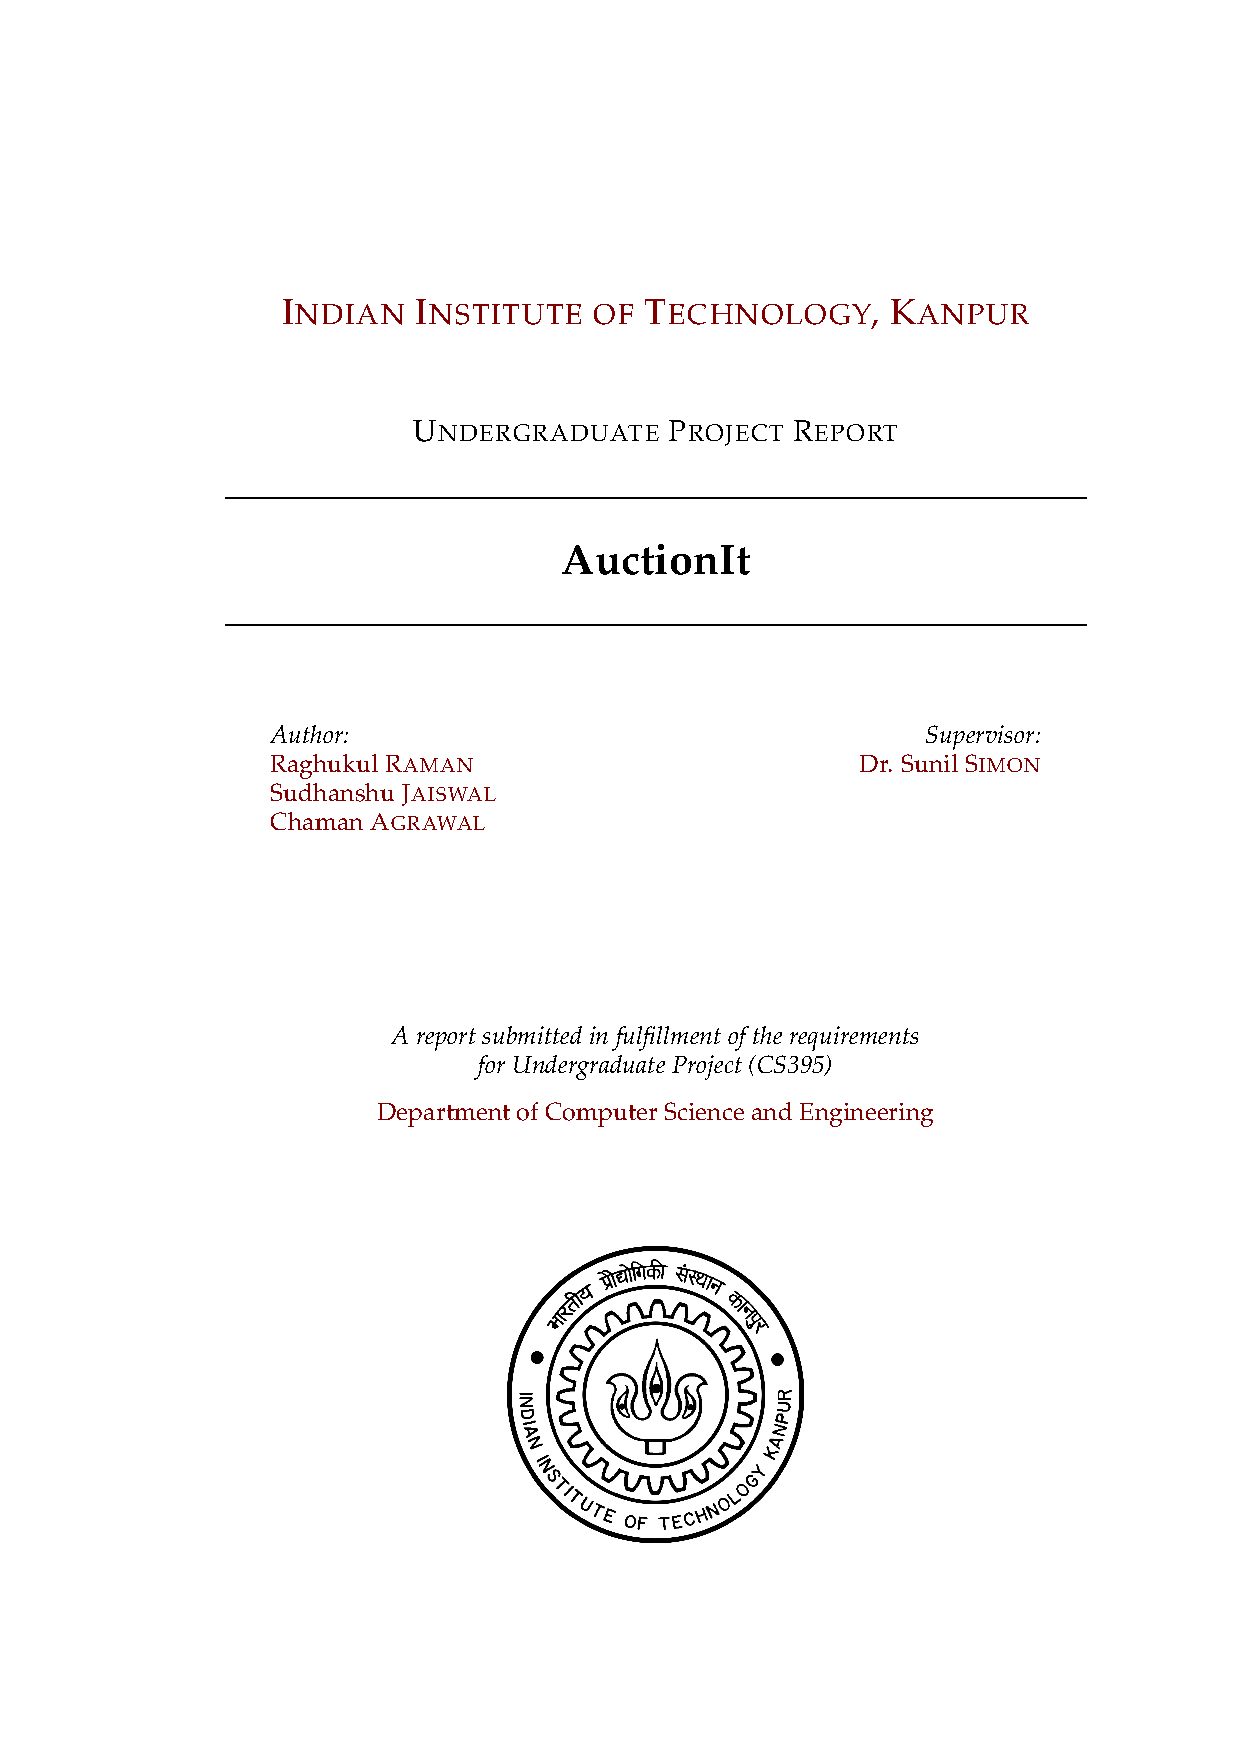
\includepdf[page={1}]{first_page.pdf}
% 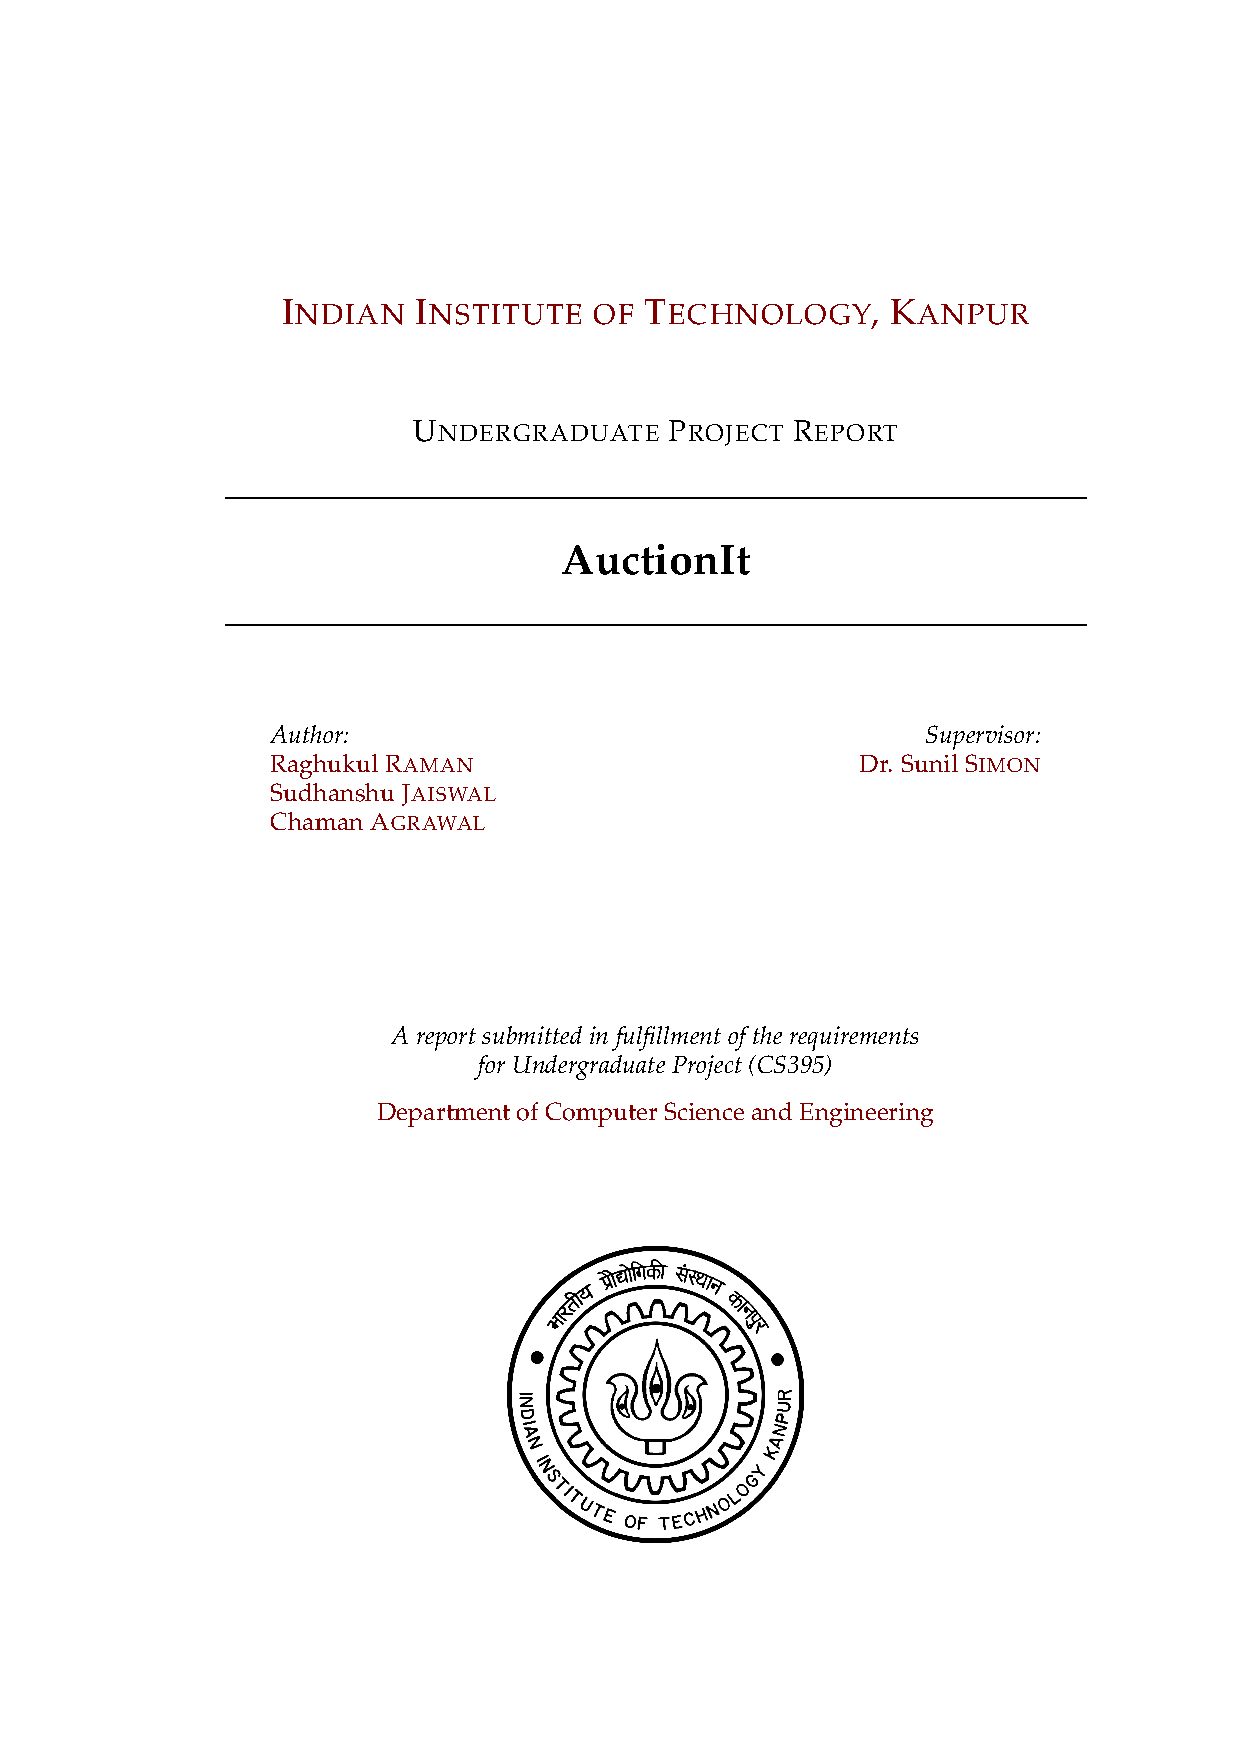
\includepdf[page={1}]{first_page.pdf}
\section*{Abstract}

% environment
% \begin{large}



An auction is a process of buying and selling goods or services by offering them up for bid, 
taking bids, and then selling the item to the highest bidder [\textit{Wiki defination}]. 
So why are auctions important? In a nutshell, it is essential because certain goods might have some value to the seller,
and therefore the seller might have some reserved price below which she would not be willing to sell.
If left to the market, the price might fall below that price.
Also, there do exist willing buyers who are ready to pay the higher value.
Moreover, it has become a method of determining prices of goods. \\
Some salient features of using an auction are \cite{vijay}:
\begin{itemize}
    \item Speedy Process, Quick Turnaround.
    \item Competitive Bidding.
    \item Auctions Work Well in Both Good and Bad Economic Times.
    \item No Negotiations.
    \item can get good idea of price.
    \item You Know Exactly When Your Property or Goods Will Be Sold.
    \item and may more...
\end{itemize}
Auctions have become an integral part of today's world; they are used extensively in almost every field. Some widely used auctions are spectrum auction, treasury auction, auction for advertisement, auctions for players such as in IPL or EPL leagues.\\ \\
Considering the need for auctions, we at this moment present a software, which is generic enough to conduct several different auctions, called \textbf{``Auctionit''}. \\
Auctionit is also useful in simulating different auctions, with data from past auctions/generated from some probability distribution. It also helps in analysis of these auctions.


\pagebreak
\section*{Introduction}
AuctionIt allows auction designers to create and host auctions; users can place bids on items in the auction and can see the results and price they have to pay at the end of the auction process.
\\\\ Auction Designers can modify and create new fields which allow them to get more data from the bidders that are relevant to the auction being held. They can also choose from pre-defined auction templates to quickly set up some of the more common auctions. They can also define their custom allocation rules and pricing rules. This allows to set up complicated rules for pricing and allocation and thus provides more freedom to the designer to create a wide variety of auctions. 
\\\\
The software categorizes auction designers and bidders as different types of users. These accounts are password protected to prevent misuse and to ensure the auction is not compromised while it runs.
\\\\
Before we started designing AuctionIt, we studied about auctions. We read papers/lectures to understand the reasons why first price and second price auctions are so popular and widely used. We also read and learned about the auction process for large-scale real-life auctions take place like treasury auctions or spectrum auctions. We read about auctions with multiple objects and how these large-scale auctions deal with having multiple objects which may be similar and how they set up rules to prevent allocating a majority of a commodity to a particular set of bidders.



\pagebreak
\thispagestyle{note_1}
\section*{Theory Review}
\subsection*{Terminologies \cite{stanford}} 
Before we proceed through formal text, let's get familiar with some of the terms.
Here bid vector \cite{stanford} $\mathbf{b} = (b_1, b_2,\ldots,b_n)$, each component represents a bid from a bidder.

\begin{itemize}
    \item[-] \textbf{Valuation:} It is the maximum price or anything equivalent to that, which denote the willingness-to-pay. 
    In general, valuations are a private entity, i.e. they are unknown to other bidders and the seller.  


    \item[-] \textbf{Sealed bid Auction:} In this kind of auctions the bids are private, or in other words, only the seller knows bids of each person.
    Bidders don't know what other bidder's bid.
    After collecting all the bids, the seller decides the winner and finally decides a selling price.
    There can be many variants of this, based on allocation rule, payment rule.\ref{temp}

    \item[-] \textbf{First-Price Auction*:} In these auctions, the highest bidder pays the price that they submit. \label{temp}

    \item[-] \textbf{Second-Price Auction*:} Allocations rule in this auction is similar to that of first price auction, i.e. Highest bidder is selected as the winner.
    However, the amount he has to pay is equal to second highest bid in the auction.
    This type of auction is also known as \textbf{Vikrey Auction} \cite{stanford}.

    \item[-] \textbf{Allocation Rule:} This rule indicates who will win the auction.
    This can be seen as a function of the bid vector.

    \item[-] \textbf{Payment Rule:} This indicates what the winner has to pay, similar to allocation rule, this can also be understood as a function of the bid vector.

    \item[-] \textbf{Dutch Auction \cite{vijay}:} This is a special type of auction in which the seller, announces an initial price for a product, and then keeps on reducing it until some buyer agrees to take it.

    \item[-] \textbf{English Auction \cite{vijay}:} This is an open bid auction (bids are present openly i.e known to other bidders), similar to the first-price auction in allocation and pricing rule.

    \item[-] \textbf{Dominant Strategy:} It refers to a strategy, which guarantees to maximize a bidders utility, independent of what other bidders bid.

    \item[-] \textbf{Utility:} It refers to the net gain after the auction is over. If the bidder wins the auction, then his utility is increased by $v_i$ (his valuation). If he loses, his net utility = $0$.
\end{itemize}
\subsection*{Second-Price Auction, DSIC and social welfare \cite{stanford}}
Second price auctions are special in the sense that there exists a dominant strategy.
Let us denote the valuations of bidder $i$ by $v_i$, his bid by $b_i$, and the bid vector by $\mathbf{b}$. Now lets shift our focus on bidder $i$, let $B = \max_{j\ne i} b_j$. 
Assume that bidder $i$ bids truly, in other words, his bid is equal to his valuation for the object. Or $b_i = v_i$

So, if $v_i < B$, then with true bidding his net utility gain $= 0$. If $v_i > B$, then he wins, and his utility $= v_i - B$

\textbf{Observation 1:} Truthful bidding gives a non-negative utility, irrespective of other bidders.  \\ \\
\textbf{Dominant-Strategy Incentive Compatible(DSIC)\cite{stanford}:} An auction is DSIC if
\begin{itemize}
    \item[-] Truthful bidding is always a dominant strategy.
    \item[-] Truthful bidders always obtain non negative utility.
\end{itemize}
\textbf{Social Welfare\cite{stanford}:} Social welfare ($\mathbf{W}$) is defined as the net welfare of society, mathematically $\mathbf{W} = \sum_{i=1}^{n}v_i x_i$. \\ \\
\textbf{Note:} Second-Price auction is DSIC and welfare maximizing.


\pagebreak
Let's now turn our attention to more complex auction: \\

\textbf{ Vickrey–Clarke–Groves (VCG) Auctions \cite{vijay}:}\\

A VCG auction is a generalization of second price (Vickrey) auctions to multiple identical items. In a VCG auction, where a set of identical items are sold, the bidders submit their sealed bids based on their internal valuations of the items. Each bidder can have multiple bids depending on the number of things they bid on; then the auction closes when all the bids are submitted.
\\
From all possible bid combinations, the one that maximizes the social welfare (sum of bids) is chosen, and the bidders receive their respective items according to the selected bid combination. Now each winner pays the amount of welfare loss (harm to other bidders) caused by his presence. \cite{sponsored}
\\
This price can be calculated as: (sum of bids of the auction from the second best combination of bids) - (what other bidders have bid in the current (best) combination of bids).


\subsection*{Treasury Securities auctions}

\textbf{Treasury securities:} Treasury securities or Treasuries are bonds issued by the government to meet their financial debts \cite{rbi}. Based on the period of maturity they are categorized into different types that are Treasury bills, notes, bonds, and Treasury inflation-protected securities.
\\\\
Most of the treasury auctions come in one of the two categories of auctions: Discriminatory Price auction and Uniform Price auction.
\\\\
\textbf{Discriminatory-Price auction:} \\In Discriminatory Price auction, allocation rule is that the bidder with the highest bid wins and the winner pays his bid, so this reduces to the first-price auction in case of a single object auction.
\\\\
\textbf{Uniform-Price auction:} \\In this, the allocation rule is same as Discriminatory Price auction, that is the winner with the highest bid wins but in this case, all winners pay an averaged uniform price, and this cuts to the second-price auction in single item auction.
\\\\
Treasury auctions are different from other auctions as the values of these securities in the secondary market in known before the auction and are independent of the private valuation of the bidders. These type of auctions are called common value auctions - this difference in valuation results in a phenomenon called 'winner's curse' which is a significant factor in choosing between the above two pricing rules for revenue maximization proper of the above two price rules.
\\\\
\textbf{Winner's Curse:}\\ In a common value auction, the real value of the item is the same for all the bidders, but they bid differently according to their estimate of the secondary market value. If we take the average of all the bids as an estimate of the actual secondary market value, then the highest bidder incurs the highest loss by winning the item at such a high price.
\\\\
From the definition of the winner's curse, it can be observed that the winning bidder will suffer more loss in the case of discriminatory price auction than uniform price auction. This causes the bidders to bid less than there valuation and results in lower revenue.
\\\\
Hence the Uniform-price method is more efficient than the Discriminatory-price method regarding revenue generation, but several surveys reveal that Discriminatory-price method dominates in Treasury auctions in most parts of the world and so this is an example of a situation where theory and practice do not agree with each other.

\pagebreak
\subsection*{US Radio spectrum reallocation}

The following is a study of the process used for the US radio spectrum reallocation given to television stations and clear spectrum for wireless internet service providers.
\\\\
The spectrum reallocation process is a complex one and needs to handle multiple challenges like how many television channels to reallocate, which channels to reassign, how to determine compensation for reassignment, how to distribute the cleared spectrum to the wireless companies etc. One of the major problems is that the channels removed and their geographical location needs to be continuous for the wireless broadband purpose. The continuity requirement of channels and their geographic location makes even small owners important, and thus each broadcaster can ask for a higher price, exploiting his/her importance for the whole project. Other than these multiple problems the computational issues are also a concern. It is computationally expensive to check for interference constraints, and these checks are required for each reassignment.
\\\\
The auction to reassign spectrum, which came to be known as the 'incentive auction', involved bidding by both buyers and sellers.
\\\\
\textbf{Incentive auction:} This consists of two separate auctions - a backward auction to determine the price at which broadcasters will sell their spectrum usage rights and a forward auction to identify the costs companies will pay for wireless allocation. Both forward and backward auctions are VCG auctions and belong to a class of deferred acceptance algorithm, forward auction's bidding increases with rounds while the back auction is a decreasing clock auction.

\subsubsection*{VCG for the incentive auction}

In a VCG auction if the price of one player is a nondecreasing function of the bid by another player then they are called substitutes on the other hand if the price is a nonincreasing function of the other player's bid then they are called complements. Aggressive bidding by substitutes is desired as it will reduce the price of the radio spectrum.
\\\\
If one does not have to care about the cost of reallocation, then VCG auction will be an optimal choice that will promote truthful bidding and maximizes revenue. Each bid independently of other bidders and since each player bids regardless of the others the dominant strategy will be to bidders to bid their valuations. In the same way, the radio station will sell his license only when the price is strictly higher than his estimate.
\\\\
In the real incentive auction, a large number of stations are needed to clear even little spectrum for nationwide usage so the cost of reallocation cannot be ignored. This problem is solved by the changed property rights of television stations. The station only has right for interference-free coverage in some channel. As a result, the price of stations reduced since if the price is too high, it can be reassigned to a different channel. This promotes competition among the channels and makes them substitutes.
\\\\
So an unmodified VCG auction is not suitable for incentive auction because:

\begin{description}

\item[$\bullet$] It generally runs a budget deficit.
\item[$\bullet$] It is computationally hard to solve the value maximization reallocation problem with millions of interference constraints subjected.
\item[$\bullet$] The success of auction depends on the participation of small broadcasters. They may find the auction mechanism complex and decline to participate at all.

\end{description}

\pagebreak
\subsubsection*{Modified VCG for the incentive auction}

A Heuristic Clock Auction for incentive auction achieves high efficiency and more straightforward computation process and still strategy-proof. The design involves bidding in two auctions: a reversed auction for government to buy broadcasting rights from radio stations and a forward auction to sell the cleared spectrum to the wireless broadcasters. In each of the auctions, the auctioneer asks players to submit offers and then iteratively rejects them one by one. The auctioneer may allow the rejected player to offer again. At the end of the auction, all the offers that are not dismissed are accepted.
\\\\
The reverse is a decreasing clock auction in which the auctioneer quotes a decreasing sequence of prices, and the players indicate if they are willing to sell at that price or not. If not they leave the auction irreversibly. When the auction ends, all the remaining players sell their rights at the last quoted price. A similar approach is used in the forward auction to sell the rights to the wireless broadcasters.



\pagebreak
\section*{Design Details}
In this section, we discuss the fabrication details for our software. 
First of all, let's get familiar with the database structure.
\subsection*{Databases}
\begin{itemize}
    \item \textbf{User Table:} This table consists1 of all the data(login details) relevant to a particular bidder.
    \begin{itemize}
        \item[-] User ID: this id is unique for each user, it is initiated by a counter value and increments on the addition of new user.
        \item[-] Login details: email ID, username, password (hashed) and salt.
        \item[-] Profile details: such as gender, date of birth etc.
        \item[-] Past auctions: this is stored in form of a list which includes all the past auction which this user has taken part in.

    \end{itemize}
    We are storing the past auctions of a bidder so that we can show his previous bids with ease, without explicitly searching in all the auction table.

    \item \textbf{Designer Table:} This table contains information of all sellers or in other words auction creators. 
    The features for a particular designer in our table are:
    \begin{itemize}
        \item[-] Designer ID: similar to the user ID.
        \item[-] All the data that we have in the user table (since a designer is also a user).
        \item[-] Past auction IDs: The auctions that this designer has created, along with the total revenue from that auction. Similar to the user table, these are also stored in form of a list of pairs.
        \item[-] Pricing and Allocation rules: These contain the pricing rule ID and allocation rule ID of the custom allocation/pricing rule, that this designer has created/used.
    \end{itemize}
    In this designer table, we explicitly store the auction ids, which this designer created in past so as to display their details, instead of checking each auction and getting all auction created by this designer explicitly. 
    Past auction will also help the designer create new auction with a slight modification of the past auctions. 
    Same applies for storing pricing and allocation rules, he can use them in new auctions.

    \item \textbf{Default Auction Table:} These include the default auction that we provide in our system. A designer can easily import them, modify some of the features and make it live! Some of the features stored in this table are:
    \begin{itemize}
        \item[-] Default auction ID: unique to each auction.
        \item[-] Ranking table address. 
        \item[-] Duration of auction.
        \item[-] Base price for the product.
        \item[-] Pricing rule: Stores the rule id for the rule which this auction uses.
        \item[-] Allocation rule: Similar to pricing rule.
        \item[-] Bid unit: Denotes the currency/mode of payment.
        \item[-] Revenue: net gain by this auction.
        \item[-] Bid step size: this signifies the net increase in bid value, in case of a tie. For example, in an English auction, the price of a good is increased in step till only one user is willing to buy.
        \item[-] Item description: quantity, brand etc.
        \item[-] Organizer details.
        \item[-] Bidder qualifying criteria: that each bidder must satisfy in order to take part in.
    \end{itemize}
    Note that some of the features listed here are only relevant to auctions which are live and running, for eg. revenue.
    \item \textbf{Live auction table:} This table stores the detail corresponding to a running auction. Some features of this table are:
    \begin{itemize}
        \item[-] Auction ID: unique to each auction.
        \item[-] Auction label: In case of a sequential auction this feature is relevant, where the subsequent auction is similar to the previous one.\cite{treasury}
        \item[-] Designer ID: user ID of the owner.
        \item[-] Creation date
        \item[-] Start / End date: denotes the duration when auction would be live.
        \item[-] features from default auction tables: since each auction is an instance of default auction with some new features.
        \item[-] Ranking table address: a pointer to the table which stores the live bids of this auction.
    \end{itemize}

    \item \textbf{Ranking table:} this stores the bids for a particular auction. Note that for each auction we'll create an instance of this table, and store the pointer to this table in the live auction table. 
    It stores:
    \begin{itemize}
        \item[-] Serial No.
        \item[-] Username
        \item[-] Bid value
    \end{itemize}
    Whenever a user wants to see the current leaderboard, we'll simply apply the allocation rule, and list out bidders in sorted order, with respect to their points.

    \item \textbf{Allocation/Pricing rule table:} two tables containing designer ID, rule ID, raw code for the rule and the rule name (optional).
\end{itemize}



\pagebreak
\begin{thebibliography}{9}

\bibitem{stanford}
Tim Roughgarden.
\textit{Lectures Notes on Algorithmic Game Theory.}
Stanford CS364A, Fall 2013.

\bibitem{vijay}
Vijay Krishna.
\textit{Auction Theory.}
Second Edition - 2010.

\bibitem{treasury} 
Leonardo Bartolini and Carlo Cottarelli.
\textit{Designing Effective Auctions for Treasury Securities}. 
Current issues in \texttt{ECONOMICS} and \texttt{FINANCE}, \textit{Vol. 3 No. 9, July 97}

\bibitem{rbi} 
Ravi Shankar and Sanjoy Bose. 
\textit{Auctions of Government Securities in India – An Analysis.}
Reserve Bank of India Occasional Papers,\textit{ Vol. 29 No. 3, Winter 2008}

\bibitem{recent_adapt}
Kenneth D. Garbade and Jeffrey F. Ingber.
\textit{The Treasury Auction Process: Objectives, Structure, and Recent Adaptations.}
Current issues in \texttt{ECONOMICS} and \texttt{FINANCE}, \textit{Vol. 11 No. 2, Feb 06}

\bibitem{}
Paul R. Milgrom.
\textit{Auctions and Bidding: A Primer.}
Journal of Economic Perspective, \textit{Vol. 3 No. 3, Summer 89}

\bibitem{competitive_bidding}
Paul R. Milgrom and Robert J. Weber.
\textit{A theory of auctions and competitive bidding - II.}
1981

\bibitem{sponsored}
Luis von Ahn.
\textit{Sponsored Search}.
Science of the Web Course Notes, \textit{15-396} - Carnegie Mellon University, Oct 2011

\bibitem{radio_spectrum}
Kevin Leyton-Brown, Paul R. Milgrom and Ilya Segal.
\textit{Economics and computer science of a radio spectrum reallocation.}
PNAS, \textit{Vol. 114 No. 28, 2017}

\bibitem{knuthwebsite} 
Paul R. Milgrom.
\textit{Business Activities.}
\\\texttt{http://www.milgrom.net/business-activities}
\end{thebibliography}
\end{document}

